\documentclass[10pt]{article}
\usepackage[margin=0.9in]{geometry}
\usepackage{booktabs,graphicx,amsmath,hyperref,enumitem}
\usepackage[font=small]{caption}
\setlist{nosep,leftmargin=1.4em}
\title{Zero-Shot Object State Tracking with LLM-Generated Attributes}
\author{ChefOST experiment (not a published result)}
\date{October 2026}
\begin{document}
\maketitle
\vspace{-1.5em}
\begin{abstract}
\noindent We track how objects change during cooking videos without any training labels. An LLM first describes each object by a few \emph{attributes} (such as a bowl's contents) and the order it expects their values to change in. A vision-language model (VLM) then reads each attribute from video frames, and a decoder lines these readings up with the expected order. On the 30 annotated MOSCATO CMU videos, frame accuracy is 0.86, against 0.52 for random guessing and 0.74 for the best guess without video (always the LLM's final value). On objects whose state changes, accuracy is 0.87 against at most 0.71 without video. Image-text similarity models (CLIP-style) used in the same way do not help.
\end{abstract}

\section{Method}
\textbf{Input:} a video (1 frame per second), the recipe name and the names of the objects to track. The method uses nothing from MOSCATO: no labels, pseudo-labels, state words or tuning.

\textbf{Step 1: the LLM defines the attributes.} For each recipe we start a fresh Claude Opus~5.5 session that sees only the recipe name and object names (no tools, project files or memory). For each object it returns 1--4 attributes, each with 2--4 possible values. Examples: a bowl's \emph{contents} is empty, raw eggs or beaten mixture; a spoon's \emph{cleanliness} is clean or egg-coated. For every attribute the LLM also gives:
\begin{itemize}
\item three short image captions per value;
\item a \emph{script}: the order it expects the values to appear in over the video (e.g.\ empty $\to$ raw eggs $\to$ beaten $\to$ empty);
\item whether the change only goes one way, plus two captions for ``object is in view''.
\end{itemize}
So the number of states per object is not fixed: at each frame the output is one value per attribute. We drew three independent LLM samples ($s_0,s_1,s_2$; 96--109 attributes across 55 recipe--object pairs) to see how much the results depend on what the LLM writes.

\textbf{Step 2: read the attributes from the video.}
\begin{itemize}
\item \emph{VLM reader (main method).} Every 6\,s, for each object, Qwen3-VL (8B, or 32B in FP8, served with vLLM) answers one multiple-choice question: is the object visible, and if so, which value does each attribute have? Asking about one object at a time is essential. When asked about all objects at once, the model often said ``not visible'' for everything. We turn the answers into a per-second score for each value: a vote of nearby visible answers, weighted by a Gaussian with $\sigma = 5$\,s, $E_{t,v}=(p_{t,v}-1/V)\min(1,W_t)$. Here $p_{t,v}$ is the vote share for value $v$, $V$ the number of values and $W_t$ the total vote weight, so the score is near zero when the object was not seen.
\item \emph{Encoder baseline.} The similarity between each frame and each value's captions, using InternVideo, SigLIP or CLIP. Scores are normalised over time and averaged over frames where the object appears to be in view.
\end{itemize}

\textbf{Step 3: decode with the script.} A left-to-right model walks through the script and picks, for each second, the script step that best fits the scores. Moving to the next step costs 1. Skipping a step, or starting late or ending early in the script, costs 4 per step. The script therefore fixes \emph{what} changes, and the video decides \emph{when}; strong evidence can still override a wrong script. For comparison we also decode without the script: (i) take the nearest keyframe's answer, or (ii) allow any value at any time, with a penalty per switch (forward-only for one-way attributes).

\section{Experiments}
\textbf{Data.} The 30 MOSCATO CMU videos with ground truth (Brownie 10, Eggs 7, Salad 6, Pizza 4, Sandwich 3), scored once per second.

\textbf{Scoring.} MOSCATO labels are free-form words (``beaten'', ``egg-covered''), not our attribute values. A separate Claude call, used \emph{only for scoring}, sees our attributes and the GT words and maps each word to the values it implies. For example, egg mixture ``solid'' $\to$ cooking state = cooked solid; a word may imply nothing. Rules:
\begin{itemize}
\item a frame counts for an attribute only if its GT words imply some value for it;
\item a prediction is correct if it matches an implied value (when two values are implied, either counts).
\end{itemize}
The map covers 89.5\% of annotated object-frames. A second mapper (Sonnet~5.5) agrees with it well: $\kappa = 0.76$ on whether a word says anything about an attribute, and 93\% identical values when both say something.

\textbf{Metrics.} A \emph{track} is one attribute of one object in one video. A track is \emph{changing} if two of its scored frames have different, non-overlapping GT values: 61 of 359 tracks are changing.
\begin{itemize}
\item \textbf{Acc}: share of all scored frames that are correct.
\item \textbf{Acc$_\Delta$}: the same, on changing tracks only.
\item \textbf{BAcc$_\Delta$}: balanced accuracy on changing tracks. Within each track we average accuracy over its GT states, then average over tracks, so a brief state counts as much as a long one. This is the strictest test of change \emph{timing}.
\end{itemize}
\textbf{No-video baselines.} Random value per frame; always the script's first value; always its last value; and the script with its steps spaced evenly over the video. Because annotators mostly label a state once it has appeared, ``last value'' is strong on Acc (0.738) but poor on changing tracks, and ``evenly spaced'' is the strongest baseline on changing tracks. Confidence intervals (95\%) in Table~\ref{tab:main} are for the gain over the evenly spaced script, from 1000 bootstrap resamples of videos.

\begin{table}[!ht]\centering\small
\resizebox{\linewidth}{!}{\begin{tabular}{lcccccc}\toprule
Method (LLM sample $s_0$) & Acc & gain CI & Acc$_\Delta$ & gain CI & BAcc$_\Delta$ & gain CI\\\midrule
No video: random value & 0.517 & & 0.553 & & 0.527 & \\
No video: script's first value & 0.076 & & 0.238 & & 0.496 & \\
No video: script's last value & 0.738 & & 0.492 & & 0.522 & \\
No video: script, evenly spaced & 0.616 & -- & 0.710 & -- & 0.712 & --\\\midrule
Encoder (InternVideo), best value per frame & 0.686 & [+.02,+.13] & 0.729 & [$-$.07,+.10] & 0.637 & [$-$.16,$-$.00]\\
Encoder + script & 0.710 & [+.04,+.16] & 0.764 & [+.00,+.11] & 0.619 & [$-$.14,$-$.05]\\
VLM 8B, nearest keyframe answer & 0.826 & [+.17,+.25] & 0.863 & [+.10,+.21] & 0.684 & [$-$.11,+.05]\\
VLM 8B + script & \textbf{0.862} & [+.20,+.28] & 0.865 & [+.09,+.22] & 0.706 & [$-$.08,+.06]\\
VLM 32B, nearest keyframe answer & 0.774 & [+.12,+.19] & 0.840 & [+.08,+.18] & 0.707 & [$-$.07,+.06]\\
VLM 32B + script & 0.810 & [+.14,+.24] & \textbf{0.866} & [+.10,+.21] & \textbf{0.733} & [$-$.04,+.08]\\
Control: VLM 8B answers from a \emph{different} video + script$^*$ & 0.820 & & 0.809 & & 0.655 & \\\midrule
Upper reference: best constant value per track (uses GT) & 0.972 & & 0.876 & & 0.541 & \\\bottomrule
\end{tabular}}
\caption{Main results: 30 videos, 359 tracks, 61 changing. Random value is the mean of 5 draws ($\pm$0.01). $^*$Mean of 5 random choices of the other video ($\pm$0.01--0.03).}\label{tab:main}
\end{table}

\textbf{Main findings (Table~\ref{tab:main}).}
\begin{itemize}
\item \emph{The VLM beats every no-video baseline on accuracy.} On Acc, VLM 8B + script is +0.12 above the best no-video baseline, the last value (CI [+.06,+.19]); with 32B it is +0.07 (CI [+.02,+.13]). On Acc$_\Delta$ it is +0.16 above the best one, the evenly spaced script (CI [+.09,+.22]).
\item \emph{Part of that gain is not specific to the video.} With VLM answers taken from a \emph{different} video of the same recipe, Acc is still 0.82. Much of the all-frame gain therefore comes from the VLM recognising each object's typical state. The video's own answers matter on changing tracks: 0.865 vs 0.809 Acc$_\Delta$, and 0.706 vs 0.655 BAcc$_\Delta$.
\item \emph{Change timing is not yet better than the script.} BAcc$_\Delta$ is not significantly above the script-only baseline (best: 32B + script, 0.733 vs 0.712).
\item \emph{Encoders do not help.} With the LLM's captions, InternVideo, SigLIP and CLIP all fall below the script on BAcc$_\Delta$ (0.62--0.66 vs 0.71). An earlier slider study found encoder gains only with captions written after looking at the labels.
\end{itemize}

\begin{table}[t]\centering\small
\resizebox{\linewidth}{!}{\begin{tabular}{lccccc}\toprule
Setting (VLM 8B unless noted) & changing tracks & Acc, last value & Acc & Acc$_\Delta$ & BAcc$_\Delta$\\\midrule
LLM sample $s_0$ & 61 & 0.738 & 0.616 / 0.862 & 0.710 / 0.865 & 0.712 / 0.706\\
LLM sample $s_1$ & 61 & 0.754 & 0.617 / 0.846 & 0.683 / 0.845 & 0.711 / 0.657\\
LLM sample $s_2$ & 57 & 0.802 & 0.619 / 0.844 & 0.712 / 0.800 & 0.701 / 0.638\\
$s_0$, scoring map by Sonnet 5.5 & 65 & 0.745 & 0.617 / 0.842 & 0.708 / 0.844 & 0.688 / 0.657\\
$s_0$, VLM 32B & 61 & 0.738 & 0.616 / 0.810 & 0.710 / 0.866 & 0.712 / 0.733\\\midrule
$s_0$, keyframes every 12 / 24 / 48\,s & 61 & 0.738 & 0.829 / 0.810 / 0.782 & 0.844 / 0.812 / 0.781 & 0.666 / 0.695 / 0.702\\\bottomrule
\end{tabular}}
\caption{Robustness. Acc, Acc$_\Delta$ and BAcc$_\Delta$ cells are \emph{evenly spaced script / VLM + script}; the last row gives VLM + script at each keyframe spacing. ``Acc, last value'' is the strongest no-video baseline on Acc.}\label{tab:rob}
\end{table}

\textbf{Robustness (Table~\ref{tab:rob}).} The Acc$_\Delta$ gain over the evenly spaced script holds for all three LLM samples, both scoring maps and both VLM sizes. The Acc gain over the last-value baseline is significant in 4 of the 5 settings; for LLM sample $s_2$ it is +0.04 and not significant (CI [$-$.02,+.12]). Reading frames less often steadily lowers accuracy.

\textbf{Where the VLM helps and where it hurts.} We split the changing tracks into two groups:
\begin{itemize}
\item \emph{Contents, fill level and location} (46 tracks; e.g.\ pan contents, baking-tray contents, where the batter is): BAcc$_\Delta$ rises from 0.670 to 0.733 with 8B (gain CI [$-$.02,+.13], not significant) and to 0.761 with 32B (gain CI [+.03,+.15], significant). See Fig.~\ref{fig:tl}.
\item \emph{Tool cleanliness} (15 tracks: spoon, knife, spatula): the VLM calls a tool ``coated'' as soon as it is used, so it misses the short clean period that annotators mark. BAcc$_\Delta$ drops by 0.20--0.30 in every setting, and the script alone does better.
\end{itemize}

\begin{figure}[h]\centering
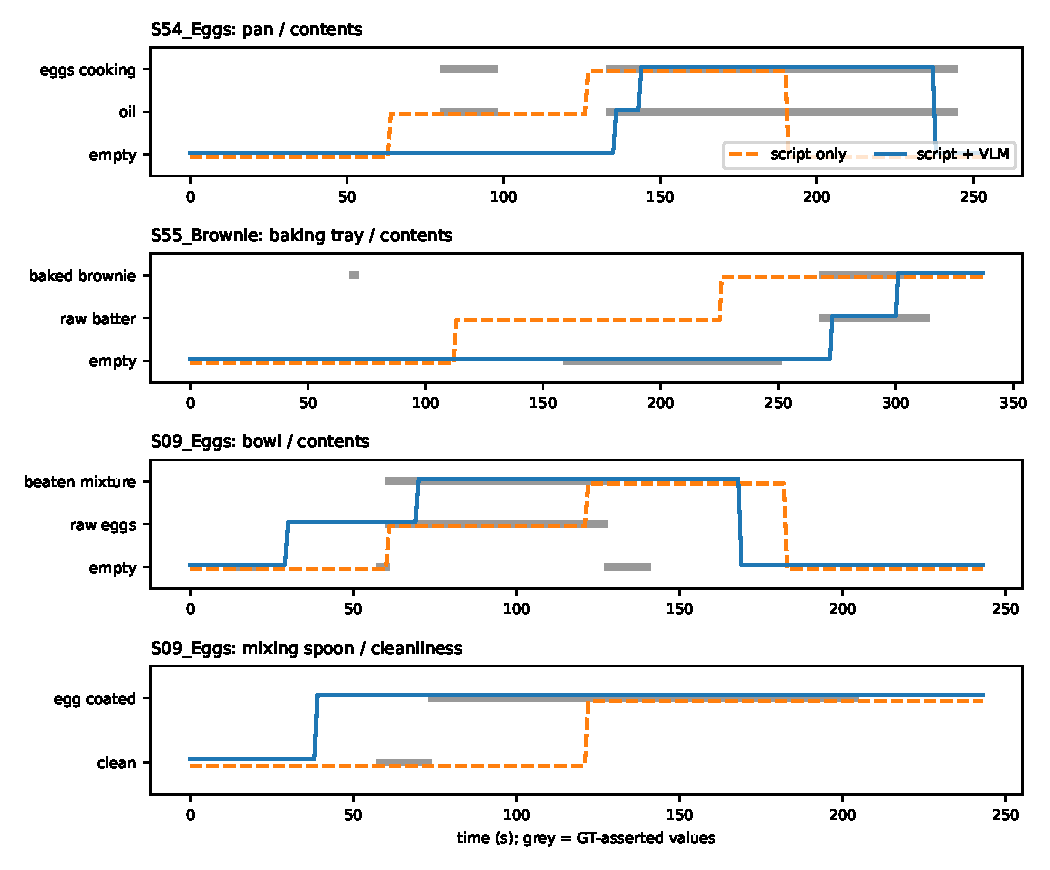
\includegraphics[width=.58\linewidth]{timelines.pdf}
\caption{VLM 32B + script (blue) vs.\ script only (orange) on four tracks. Grey: values implied by the GT words (some frames have two). The bottom row shows the cleanliness failure.}\label{fig:tl}
\end{figure}

\section{Conclusion}
From only the recipe and object names, an LLM can define a useful state space for each object: its attributes, their values and the expected order of change. A VLM that reads those attributes from keyframes, decoded along that order, tracks object states with no training labels. On MOSCATO CMU it reaches 0.86 frame accuracy, above random guessing (0.52) and the best no-video guess (0.74), and 0.87 on changing objects (best no-video: 0.71). These gains are mostly consistent across LLM samples, scoring maps and VLM sizes. CLIP-style similarity with the same captions does not help.

Two limits remain. The timing of short states is not yet better than the script alone, mostly because of tool cleanliness. And part of the gain reflects what is typical for the recipe rather than what happens in the specific video. Next steps: query the VLM more densely, or on short clips, around predicted changes; crop small tools before asking; and agree as a team whether the scoring-only word-to-value map is acceptable.

Code: \texttt{vidosc/experiments/attrs/}. W\&B: group \texttt{attrs} in \texttt{chefOST/vidosc-experiments}.
\end{document}
